\documentclass[12pt, a4paper]{article}

\usepackage{amsmath, amssymb, amsthm}
\usepackage{geometry}
\usepackage{booktabs}
\usepackage{array}
\usepackage{hyperref}
\usepackage{xcolor}
\usepackage{tcolorbox}
\usepackage{enumitem}
\usepackage{parskip}
\usepackage{tikz}
\usetikzlibrary{arrows.meta, positioning, calc}

\geometry{margin=2.5cm}

\newif\ifstudentmode
\studentmodefalse
\ifx\studentflag\undefined\else\studentmodetrue\fi

\newcommand{\sol}[2][6cm]{%
  \ifstudentmode\underline{\hspace{#1}}\else{#2}\fi}
\newcommand{\soleq}[2][3cm]{%
  \ifstudentmode
    \par\vspace{4pt}\noindent\rule{\linewidth}{0.5pt}\\[#1]%
    \noindent\rule{\linewidth}{0.5pt}\par\vspace{4pt}%
  \else\[#2\]\fi}

\definecolor{mainblue}{RGB}{30, 100, 180}
\definecolor{boxbg}{RGB}{235, 243, 255}
\definecolor{notebg}{RGB}{255, 248, 230}
\definecolor{warnbg}{RGB}{255, 235, 235}
\definecolor{greenbg}{RGB}{230, 255, 235}
\definecolor{purplebg}{RGB}{245, 235, 255}

\tcbuselibrary{skins, breakable}

\newtcolorbox{resultbox}{colback=boxbg,colframe=mainblue,boxrule=1.2pt,arc=4pt,
  title={Result},fonttitle=\bfseries\color{white},coltitle=white,
  attach boxed title to top left={yshift=-2mm,xshift=4mm},
  boxed title style={colback=mainblue,arc=3pt}}

\newtcolorbox{notebox}{colback=notebg,colframe=orange!70!black,
  boxrule=1pt,arc=4pt,left=4pt,right=4pt}

\newtcolorbox{warnbox}{colback=warnbg,colframe=red!60!black,
  boxrule=1pt,arc=4pt,left=4pt,right=4pt}

\newtcolorbox{stepbox}[1]{colback=greenbg,colframe=green!50!black,
  boxrule=1pt,arc=4pt,title={#1},fonttitle=\bfseries,coltitle=green!30!black}

\newtcolorbox{keybox}{colback=purplebg,colframe=purple!60!black,
  boxrule=1pt,arc=4pt,left=4pt,right=4pt}

\theoremstyle{definition}
\newtheorem{example}{Example}[section]

\begin{document}

\begin{center}
  {\LARGE \textbf{Section 4.5: Weight Initialisation \& Learning Rate Schedules}} \\[0.3em]
  {\large\itshape Starting Right and Slowing Down at the Right Time} \\[0.5em]
  {\large AI Class --- Lecture Notes}%
  \ifstudentmode\quad{\normalsize\color{gray}[Student Copy]}\fi
\end{center}

\vspace{1em}\hrule\vspace{1.5em}

% ══════════════════════════════════════════════════════════════════════════════
\section{Part A: Weight Initialisation}

% ──────────────────────────────────────────────────────────────────────────────
\subsection{Why Initialisation Matters}

Before training begins, every weight must be given a starting value.
This seemingly minor choice can make the difference between a network
that trains well and one that never learns at all.

\subsubsection*{The All-Zeros Failure}

Suppose every weight in a layer is initialised to zero.

\begin{warnbox}
\textbf{Symmetry problem.}
If all weights in a layer are equal, every neuron in that layer computes
\emph{exactly the same} pre-activation.
They receive \emph{exactly the same} gradient.
They update to \emph{exactly the same} new value.

The layer is stuck: no matter how long training runs, all neurons remain
identical.  A hidden layer of $n$ neurons collapses to a single effective
neuron --- the network has no more capacity than a much smaller one.
\end{warnbox}

\textbf{Small random values} break this symmetry: each neuron starts with
a different weight, so gradients differ and neurons specialise.
But if the values are \emph{too large}, activations saturate and gradients
vanish.  We need weights that are random \emph{and} appropriately scaled.

% ──────────────────────────────────────────────────────────────────────────────
\subsection{Xavier (Glorot) Initialisation --- for Sigmoid / Tanh}

\begin{resultbox}
Draw each weight uniformly:
\[
  w \;\sim\; \mathcal{U}\!\left[-\frac{\sqrt{6}}{\sqrt{n_{\text{in}}+n_{\text{out}}}},\;
                                  \frac{\sqrt{6}}{\sqrt{n_{\text{in}}+n_{\text{out}}}}\right]
\]
where $n_{\text{in}}$ is the number of inputs to the layer and
$n_{\text{out}}$ is the number of outputs.
\end{resultbox}

\textbf{Intuition.}
Xavier init keeps the variance of activations and gradients roughly equal
across layers.  If signals grow layer by layer, deep networks explode;
if they shrink, they vanish.  Xavier targets the sweet spot for
linear-ish activations (sigmoid near $0$, tanh).

\subsubsection*{Numerical Example}

For our 2-hidden-neuron layer: $n_{\text{in}} = 2$, $n_{\text{out}} = 2$.

\begin{stepbox}{Compute the range}
\[
  \text{limit} = \frac{\sqrt{6}}{\sqrt{n_{\text{in}}+n_{\text{out}}}}
               = \frac{\sqrt{6}}{\sqrt{4}}
               = \frac{2.449}{2}
               = \sol[3cm]{1.225}
\]
\end{stepbox}

Each weight is drawn from $\mathcal{U}[-1.225,\; 1.225]$.
For the output layer ($n_{\text{in}}=2$, $n_{\text{out}}=1$):
\[
  \text{limit} = \frac{\sqrt{6}}{\sqrt{3}} = \sqrt{2} \approx \sol[3cm]{1.414}
\]

% ──────────────────────────────────────────────────────────────────────────────
\subsection{He (Kaiming) Initialisation --- for ReLU}

ReLU sets half its inputs to zero, effectively halving the variance.
He init corrects for this:

\begin{resultbox}
Draw each weight from a normal distribution:
\[
  w \;\sim\; \mathcal{N}\!\left(0,\;\frac{2}{n_{\text{in}}}\right)
  \qquad\Longleftrightarrow\qquad
  w = \sqrt{\frac{2}{n_{\text{in}}}}\;\cdot\;\mathcal{N}(0,1)
\]
\end{resultbox}

\subsubsection*{Numerical Example}

For a ReLU layer with $n_{\text{in}} = 2$:
\[
  \sigma_w = \sqrt{\frac{2}{n_{\text{in}}}} = \sqrt{\frac{2}{2}} = \sol[3cm]{1.000}
\]

Weights are drawn from $\mathcal{N}(0, 1)$ --- standard normal.

For a larger layer with $n_{\text{in}} = 512$:
\[
  \sigma_w = \sqrt{\frac{2}{512}} = \sqrt{0.00391} \approx \sol[3cm]{0.0625}
\]

Each incoming connection contributes less variance as the fan-in grows.

% ──────────────────────────────────────────────────────────────────────────────
\subsection{Comparison Table}

\begin{center}
\renewcommand{\arraystretch}{1.3}
\begin{tabular}{llll}
\toprule
Method & Distribution & Scale & Activation \\
\midrule
Zeros  & $w = 0$ & --- & \textbf{Never use} \\
Xavier & Uniform & $\pm\sqrt{6/(n_{\text{in}}+n_{\text{out}})}$ & Sigmoid, Tanh \\
He     & Normal  & $\mathcal{N}(0,\,2/n_{\text{in}})$ & ReLU and variants \\
\bottomrule
\end{tabular}
\end{center}

\begin{notebox}
\textbf{PyTorch.}
\begin{verbatim}
nn.init.xavier_uniform_(layer.weight)   # Xavier
nn.init.kaiming_normal_(layer.weight)   # He (default: ReLU mode)
\end{verbatim}
PyTorch's default initialisation uses Kaiming uniform, which works
reasonably well in most cases.
See \texttt{code\_examples.py} for a complete model with explicit init.
\end{notebox}

% ══════════════════════════════════════════════════════════════════════════════
\section{Part B: Learning Rate Schedules}

% ──────────────────────────────────────────────────────────────────────────────
\subsection{Why a Fixed Learning Rate is Not Always Best}

\begin{center}
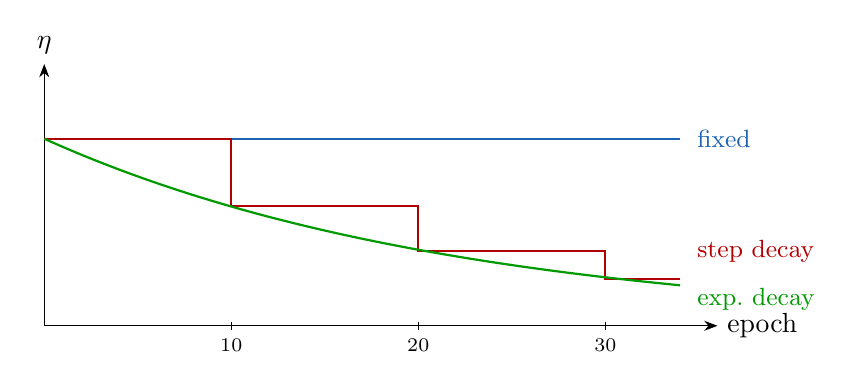
\begin{tikzpicture}[scale=0.95, >=Stealth]
  \draw[->] (0,0) -- (9,0) node[right] {epoch};
  \draw[->] (0,0) -- (0,3.5) node[above] {$\eta$};

  % Fixed LR
  \draw[thick, mainblue] (0,2.5) -- (8.5,2.5);
  \node[right, mainblue, font=\small] at (8.6,2.5) {fixed};

  % Step decay
  \draw[thick, red!70!black] (0,2.5) -- (2.5,2.5)
                              -- (2.5,1.6) -- (5.0,1.6)
                              -- (5.0,1.0) -- (7.5,1.0)
                              -- (7.5,0.63) -- (8.5,0.63);
  \node[right, red!70!black, font=\small] at (8.6,1.0) {step decay};

  % Exponential decay
  \draw[thick, green!60!black, domain=0:8.5, samples=100]
    plot (\x, {2.5*exp(-0.18*\x)});
  \node[right, green!60!black, font=\small] at (8.6,0.35) {exp.\ decay};

  % Axis ticks
  \foreach \e/\x in {10/2.5, 20/5.0, 30/7.5}
    \draw (\x,0.05) -- (\x,-0.05) node[below,font=\scriptsize] {\e};
\end{tikzpicture}
\end{center}

A large learning rate early in training takes big steps toward the minimum
--- fast progress.
But near the minimum, large steps overshoot and oscillate.
\textbf{Decreasing} $\eta$ over time: fast at the start, precise at the end.

% ──────────────────────────────────────────────────────────────────────────────
\subsection{Step Decay}

Reduce the learning rate by a fixed factor every $k$ epochs:

\begin{resultbox}
\[
  \eta_t = \eta_0 \times \gamma^{\,\lfloor t / k \rfloor}
\]
where $\eta_0$ is the initial rate, $\gamma \in (0,1)$ is the decay factor,
and $k$ is the step size (epochs between drops).
\end{resultbox}

\subsubsection*{Numerical Example}

$\eta_0 = 0.1$, \; $\gamma = 0.5$, \; $k = 10$ epochs.

\begin{center}
\renewcommand{\arraystretch}{1.3}
\begin{tabular}{ccc}
\toprule
Epoch $t$ & $\lfloor t/k \rfloor$ & $\eta_t$ \\
\midrule
1--9   & 0 & $0.1 \times 0.5^0 = \sol[3cm]{0.100}$ \\
10--19 & 1 & $0.1 \times 0.5^1 = \sol[3cm]{0.050}$ \\
20--29 & 2 & $0.1 \times 0.5^2 = \sol[3cm]{0.025}$ \\
30--39 & 3 & $0.1 \times 0.5^3 = \sol[3cm]{0.0125}$ \\
\bottomrule
\end{tabular}
\end{center}

The rate halves every 10 epochs.  Training stays aggressive early, then
fine-tunes once close to the minimum.

% ──────────────────────────────────────────────────────────────────────────────
\subsection{Exponential Decay}

Reduce the learning rate smoothly every epoch:

\begin{resultbox}
\[
  \eta_t = \eta_0 \times \gamma^{\,t}
\]
Equivalently, $\eta_t = \eta_0 \, e^{-\lambda t}$ where $\lambda = -\ln \gamma$.
\end{resultbox}

\subsubsection*{Numerical Example}

$\eta_0 = 0.1$, \; $\gamma = 0.95$ (5\% decay per epoch).

\begin{center}
\renewcommand{\arraystretch}{1.3}
\begin{tabular}{ccc}
\toprule
Epoch $t$ & Formula & $\eta_t$ \\
\midrule
0  & $0.1 \times 0.95^{0}$  & $\sol[3cm]{0.1000}$ \\
5  & $0.1 \times 0.95^{5}$  & $\sol[3cm]{0.0774}$ \\
10 & $0.1 \times 0.95^{10}$ & $\sol[3cm]{0.0599}$ \\
20 & $0.1 \times 0.95^{20}$ & $\sol[3cm]{0.0358}$ \\
50 & $0.1 \times 0.95^{50}$ & $\sol[3cm]{0.0077}$ \\
\bottomrule
\end{tabular}
\end{center}

The decay is smooth rather than sudden.  $\gamma=0.95$ is a common
starting point; $\gamma=0.99$ gives a very slow decay.

% ──────────────────────────────────────────────────────────────────────────────
\subsection{Comparison}

\begin{center}
\renewcommand{\arraystretch}{1.3}
\begin{tabular}{llll}
\toprule
Schedule & Shape & Tuning & Typical use \\
\midrule
Fixed          & Flat      & Just $\eta_0$            & Quick experiments \\
Step decay     & Staircase & $\eta_0$, $\gamma$, $k$  & CV, most common \\
Exponential    & Smooth    & $\eta_0$, $\gamma$        & Smooth convergence \\
\bottomrule
\end{tabular}
\end{center}

\begin{keybox}
\textbf{Rule of thumb.}
Start with a fixed rate to confirm the model learns at all.
Add a step or exponential schedule once the architecture is finalised ---
it almost always improves the final validation loss at no extra cost.
\end{keybox}

\begin{notebox}
\textbf{PyTorch.}
\begin{verbatim}
from torch.optim.lr_scheduler import StepLR, ExponentialLR

scheduler = StepLR(optimizer, step_size=10, gamma=0.5)
scheduler = ExponentialLR(optimizer, gamma=0.95)

# Inside the training loop, after optimizer.step():
scheduler.step()
\end{verbatim}
See \texttt{code\_examples.py} for a complete training loop with a scheduler.
\end{notebox}

\end{document}
